\subsection{Recruitment Variability and Bias Correction}
\hypertarget{BiasCorrect}{}

Recruitments are defined as lognormal deviates around a log-bias adjusted spawner-recruitment curve.  The magnitude of the log-bias adjustment is calculated from the level of $\sigma_R$ , which is the standard deviation of the recruitment deviations (in log-space).  There are 5 segments of the time series in which to consider the effect of the log-bias adjustment: virgin; initial equilibrium; early data-poor period; data-rich period; very-recent/forecast. The choice of break points between these segments need not correspond directly with the settings for the bias adjustment, although some alignment might be desired. \citet{methot-adjusting-2011} provide more detailed discussion of the bias adjustment than what is provided below but do not address the separation of time periods into separate segments. The approach is illustrated with figures associated the assessment for darkblotched rockfish \citep{gertseva-status-2013}.

\begin{figure}[H]
	\begin{center}
		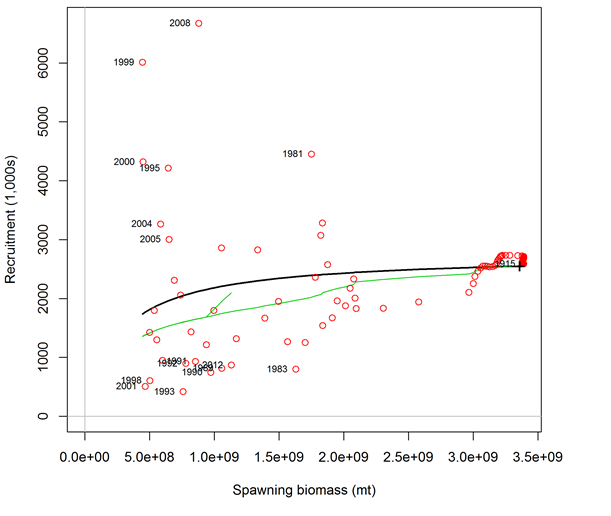
\includegraphics[scale = 0.70]{appendixA_recruits}\\
	\end{center}	
	\caption{Spawner-recruitment relationship for dark-blotched rockfish \citep{gertseva-status-2013}. Red points represent estimated recruitments, the solid black line is the stock-recruit relationship and the green line represents the adjustment to this relationship after adjustment to account for the lognormal distribution associated with each year. The "+" symbol labeled 1915 near the right side represents both the virgin and initial equilibrium of the model. The numerous red points close to the initial conditions correspond to the early years of the model with low harvest rates.}
	\label{fig:recruits}	
\end{figure}

\begin{figure}[H]
	\begin{center}
		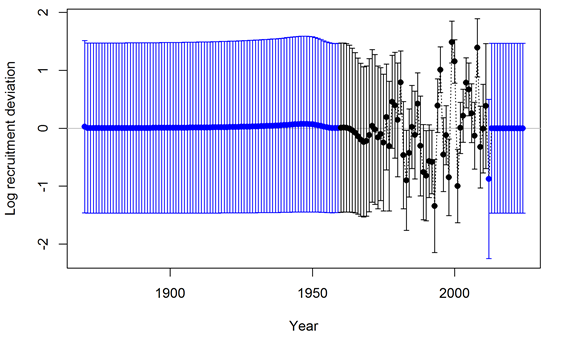
\includegraphics[scale = 0.90]{appendixA_logdevs}\\
	\end{center}
\caption{ Time series of log recruitment deviations for darkblotched rockfish with 95\% uncertainty intervals. The start year of the model is 1915, but recruitment deviations are estimated starting in 1870. The 45 deviation estimates for 1870–1914 inform the age structure used in the start year. The black color for the years 1960–2011 indicates the "main" recruitment deviation vector, while the blue color for the years 1870–1959 and 2012–2024 indicates the "early" and "late/forecast" recruitment deviation vectors, respectively.}
\label{fig:recdevs}
\end{figure}

\myparagraph{Virgin Biomass}
The R0 level of recruitment is a parameter of the spawner-recruitment curve.  This recruitment and the corresponding spawning biomass are expected to represent the long-term arithmetic mean.

\myparagraph{Initial Equilibrium}
The level of recruitment is typically maintained at the R0 level even though the initial equilibrium catch will reduce the spawning biomass below the virgin level. If steepness is moderately low or the initial F is high, then the lack of response in recruitment level may appear paradoxical. The logic is that building in the spawner-recruitment response to initial F would significantly complicate the calculations and would imply that the initial equilibrium catch level had been going on for multiple generations. If the lack of response is considered to be problematic in a particular application, then start the model at an earlier year and with a lower initial equilibrium catch so that the dynamics of the spawner-recruitment response get captured in the early period, rather than getting lost in the initial equilibrium.

\myparagraph{Early Data-Poor Period}
This is the early part of the time series where the only data typically are landed catch. There are no data to inform the model about the specific year-to-year fluctuations in recruitment, although the ending years of this period will begin to be influenced by the data.  The "early time period" is not a formal concept. It is up to the user to decide whether to start estimating recruitment deviations beginning with the first year of the model, or to delay such estimation until the data become more informative. Modeling recruitment deviations in this period may lead to a more realistic portrayal of the uncertainty in depletion, but can also lead to spurious patterns in estimated recruitments that may be driven by the fit to index data or other sources that would not be expected to have accurate information on recruitment.
	\begin{itemize}
		\item Option A: Do not estimate recruitment deviations during this early period.  During years prior to the first year of recruitment deviations, the model will set the recruitment equal to the level of the spawner-recruitment curve.  Thus, it is a mean-based level of recruitment.  Because these annual parameters are fixed to the level of the spawner-recruitment curve, they have no additional uncertainty and make no contribution to the variance of the model. This approach may produce relatively large, or small, magnitude deviations at the very beginning of the subsequent period, as the model "catches up" to any slight signal that could not be captured through estimated deviations in the early data-poor period.  There may be some effect on the estimate of R0 as a result of lack of model flexibility in balancing early period removals with signal in the early portion of the data-rich period.  
		\item Option B: Estimate recruitment deviations for all the early years. Each of these recruitment deviations is now a deviation parameter so will have a variance that contributes to the total model variance. The estimated standard deviation of each of these deviation parameters should be similar to $\sigma_R$ because $\sigma_R$ is the only constraint on these parameters (however, the last few in the sequence will begin to feel the effect of the data so may have lower standard deviations). 		
	\end{itemize}
	
\myparagraph{Data-Rich Period}
Here the length and or age data inform the model on the year-to-year level of recruitment.  These fluctuations in recruitment are assumed to have a lognormal distribution around the log-bias adjusted spawner-recruitment curve.  The level of $\sigma_R$ input to the model should match this level of fluctuation to a reasonable degree.  Because the recruitments are lognormal, they produce a mean biomass level that is comparable to the virgin biomass and thus the depletion level can be calculated without bias.  However, if the early period has recruitment deviations estimated by maximum posterior density, then the depletion levels during the early part of the data-rich period may have some lingering effect of negative bias during the early time period. The level of $\sigma_R$ should be at least as large as the level of variability in these estimated recruitments.  If too high a level of $\sigma_R$ is used, then a bias can occur in the estimate of spawner-recruitment steepness, which determines the trend in recruitment.  This occurs when the early recruitments are taken directly from the spawner- recruitment curve, so are mean unbiased, then the later recruitments are estimated as deviations from the log-bias adjusted curve.  If $\sigma_R$ is too large, then the bias-adjustment is too large, and the model may compensate by increasing steepness to keep the mean level of recent recruitments at the correct level.

\myparagraph{Recent Years/Forecast}
Here the situation is very similar to the early time period in that there are no data to inform the model about the year-to-year pattern in recruitment fluctuations so all deviations will be pulled to a zero level in the maximum posterior density.  The structure of SS3 creates no sharp dividing line between the estimation period and the forecast period.  In many cases one or more recruitments at the end of the time series will lack appreciable signal in the data and should therefore be treated as forecast recruit deviations.  To the degree that some variability is observed in these recruitments, partial or full bias correction may be desirable for these deviations separate from the purely forecast deviations, there is therefore an additional control for the level of bias correction applied to forecast deviations occurring prior to end year + 1.

\begin{figure}[H]
	\begin{center}
	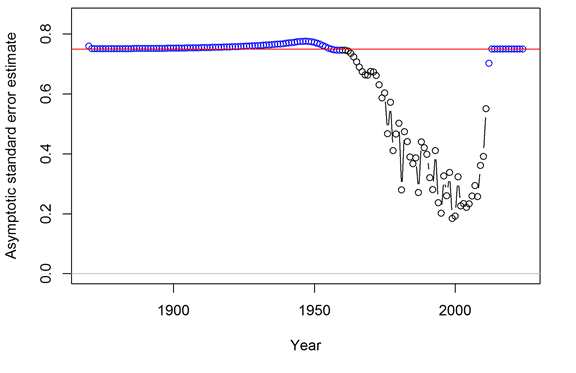
\includegraphics[scale = 0.90]{appendixA_asymerror}\\
	\end{center}
	\caption{ Timeseries of standard error estimates for the log recruitment deviations for darkblotched rockfish with 95\% uncertainty intervals. As in Figure \ref{fig:recdevs}, the black color indicates the main recruitment period. This period with lower standard error is associated with higher variability among deviations (Figure \ref{fig:recdevs}). The red line at 0.75 indicates the  $\sigma_R$ value in this model.}
	\label{fig:recSE}
\end{figure}


\begin{figure}[H]
	\begin{center}
	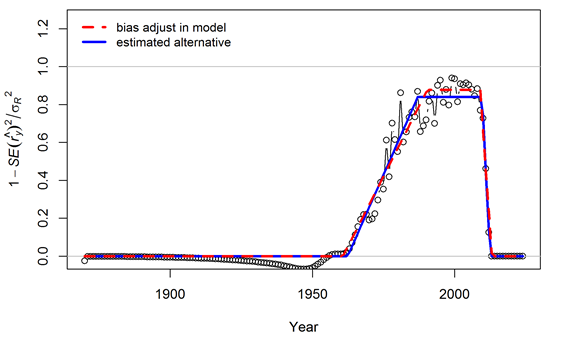
\includegraphics[scale = 0.90]{appendixA_biasadj}\\
	\end{center}
	\caption{ Transformation of the standard error estimates (shown in Figure \ref{fig:recSE}) for darkblotched rockfish following the approach suggested by \citet{methot-adjusting-2011}. These values were used to set the 5 values controlling the degree of bias adjustment (as a fraction of  $\sigma_R/2$) to account for differences in the mean and median of the lognormal distribution from which the recruitment deviations are drawn. The red line indicates a bias adjustment of 0 up to the  1960.75, ramping up to a maximum adjustment level of 0.877 for the period 1990.4–2008.98,and reducing back to 0 starting in 2013.08. Note that these values controlling the bias adjustment need not be integer year values. Also the break points in the bias adjustment function need not match the break points between early, main, and late/forecast recruitment deviation vectors (indicated by blue and black colors in Figures \ref{fig:recdevs} and \ref{fig:recSE}). The blue line indicates a functional form that minimizes the sum of squared differences between the bias adjustment function and the transformed standard error values. The subtle differences between red and blue lines are unlikely to have any appreciable effect on the model results.}
	\label{fig:ramp}
\end{figure}


\begin{figure}[H]
	\begin{center}
	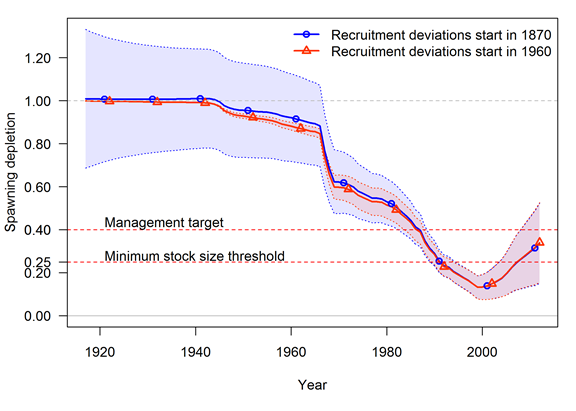
\includegraphics[scale = 0.90]{appendixA_depl}\\
	\end{center}
	\caption{ Comparison of timeseries of spawning depletion for darkblotched rockfish models with early recruitment deviations (starting in 1870) and without early deviations (only main recruitment deviations starting in 1960). The point estimates are similar, but the 95\% uncertainty intervals are substantially different. With no recruitment deviations for the early period, the estimates of spawning depletion in the early years are very precise and uncertainty increases as the stock moves into the data rich period. In contrast, the addition of the early recruitment deviations results in a large uncertainty in spawning depletion for the early years and an increase in precision as the stock moves into the data rich period. In this application, the uncertainty associated with the recent years is independent of the assumptions about early recruitments.}
\end{figure}

\myparagraph{Issues with Including Environmental Effects}
The expected level of recruitment is a function of spawning biomass, an environmental time series, and a log-bias adjustment.
\begin{equation}
	E(Recruitment) = f(SpBio) * exp(\beta*envdata) * exp(-0.5*\sigma_R^2)
\end{equation}
$\sigma_R$ is the variability of the deviations, so it is in addition to the variance "created" by the environmental effect.  So, as more of the total recruitment variability is explained by the environmental effect, the residual $\sigma_R$ should be decreased.  The model does not do this automatically.

The environmental effect is inherently lognormal.  So when an environmental effect is included in the model, the arithmetic mean recruitment level will be increased above the level predicted by f(SpBio) alone.  The consequences of this have not yet been thoroughly investigated, but there probably should be another bias correction based on the variability of the environmental data as scaled by the estimated linkage parameter, $\beta$.  It is also problematic that the environmental effect time series used as input is assumed to be measured without error.

The preferred approach to including environmental effects on recruitment is not to use the environmental effect in the direct calculation of the expected level of recruitment.  Instead, the environmental data would be used as if it was a survey observation of the recruitment deviation.  This approach is similar to using the environmental index as if it was a survey of age 0 recruitment abundance because by focusing on the fit to the deviations it removes the effect of SpBio on recruitment.  In this alternative, the $\sigma_R$ would not be changed by the environmental data; instead the environmental data would be used to explain some of the total variability represented by $\sigma_R$.  This approach may also allow greater uncertainty in forecasts, as the variability in projected recruitments would reflect both the uncertainty in the environmental observations themselves and the model fit to these observations.

\myparagraph{Initial Age Composition}
If the first year with recruitment deviations is set less than the start year of the model, then these early deviations will modify the initial age composition.  The amount of information on historical recruitment variability certainly will degrade as the model attempts to estimate deviations for older age groups in the initial equilibrium.  So the degree of bias correction is reduced linearly in proportion to age so that the correction disappears when maximum age is reached.  The initial age composition approach normally produces a result that is indistinguishable from a configuration that starts earlier in the time series and estimates a longer time series of recruitments.  However, because the initial equilibrium is calculated from a recruitment level unaffected by spawner-recruitment steepness and initial age composition adjustments are applied after the initial equilibrium is calculated, it is possible that the initial age composition approach will produce a slightly different result than if the time series was started earlier and the deviations were being applied to the recruitment levels predicted from the spawner-recruitment curve. 
